\section{Experiments}
\label{sec:experiments}

%List of questions that we want to answer.
In our experiments, we aim to answer the following questions:
\begin{enumerate}
    \item How does a state-of-the-art navigation model (CLIP + LSTM + PPO) behave in a not-so-complex maze-based environment?
    See section~\ref{subsec:miniworld-maze-results}.
    \item What is the real impact of reward shaping and $\epsilon\text{-}greedy$ techniques on such a model?
    See section~\ref{subsec:miniworld-maze-results}.
    \item When faced with a more realistic robotic navigation scenario, such as the one proposed with HM3D~\cite{ramakrishnan2021} dataset scenes in Habitat~\cite{szot2021}, what is the performance of the model under analysis?
    \item Qualitatively, how does the model navigate through the proposed environments?
    \item Is it feasible to provide clear experimental comparison environments to establish benchmarks between different RL-based visual semantic navigation models?
\end{enumerate}

\subsection{Experimental setup}\label{subsec:experimental-setup}



\paragraph{Navigation benchmarks}
%Define the two scenarios we propose: Maze and Habitat. Justify why the are interesting.
%The first environment we face is Miniwolrd-Maze from \textit{gym-miniworld}~\cite{gym_miniworld}.
We conducted our main experimentation in the Miniwolrd-Maze environment from \textit{gym-miniworld}~\cite{gym_miniworld}.
This is a minimalistic 3D interior environment simulator for RL and robotics, where 3D mazes can be procedurally generated.
In this benchmark, the agent receives an egocentric 3D view of the environment and has to navigate to a red cube representing the target.
A schematic top-view representation can be found in figure~\ref{fig:graphical_abstract}.
We propose two configurations, Maze-S3 and Maze-S5, that correspond to a $3\times3$ and $5\times5$ tiles maze environments, respectively.
The agent and the target are initialized in opposite corners of the Maze, and in every episode, a new wall distribution is randomly generated.
The action space $\mathcal{A}$ consists of the following actions: $move\_forward$, $turn\_left$, $turn\_right$.
To establish future comparisons with new navigation models in this benchmark, we provide 100 procedurally generated mazes and use them as a separate test set.


The second environment is AI Habitat~\cite{szot2021}, which allows for the training of embodied AI agents, such as virtual robots, in a highly photorealistic and efficient 3D simulator.
This scenario is particularly relevant because it will allow us to evaluate how a robot would behave in a more realistic navigation scenario than the one posed with the mazes.
We use one 3D scene from HM3D~\cite{ramakrishnan2021} dataset (see figure~\ref{fig:dollhouse}).
%This dataset consists of 3D reconstructions from real-world locations and posses state-of-the-art visual fidelity.
We follow an \textit{oracle stop} configuration in Habitat, in which the environment is in charge of telling the agent when to stop, so the action space $\mathcal{A}$ consists of the following actions: $move\_forward$, $turn\_left$, $turn\_right$, $look\_up$ and $look\_down$.

As for the evaluation metrics, we evaluate the Maze models using Success Rate (SR) and Steps Per Episode (SPE) metrics.
Additionally, for Habitat models we also employ Shortest Path Length (SPL) and Distance To Goal (DTG).
All these are the standard metrics for the ObjectNav problem in Habitat Challenge~\cite{batra2020}.

\paragraph{Implementation details}
%Provide the details of the benchmark we propose: description of PyRIL, models for navigation, implementation details that can help others to replicate/understand the results.
We leverage on the state-of-the-art RL approach for embodied navigation in \cite{khandelwal2022} with some minor simplifications.
As it is shown in figure~\ref{fig:network_clip_diagram}, the first part of our model consists in a pre-trained CLIP plus RestNet50 module as feature extractor, which receives an RGB image and produces a latent vector of size 1024.
We then compute the embeddings for the last 10 time steps and pass them through an LSTM layer with 128 neurons.
Finally, we concatenate two hidden linear layers of 128 neurons with a tanh unit for activation.
Our agent has two separate networks, one for the actor and one for the critic.
Both networks share the feature extractor.
The output layer of the actor consists in a linear layer of the same dimension as the number of actions with a softmax function.
The output layer of the critic consists in a linear layer with one neuron and linear activation.

We use the PPO~\cite{schulman2017} agent provided by pyRIL reinforcement learning library~\cite{pyRIL}.
This is a lightweight python library which contains a collection of state-of-the-art deep reinforcement and imitation learning methods, environment wrappers, modularity and different prototyping options.

As our codes are publicly released, we provide a set of tools to improve the reproducibility of RL experiments, with clear and standardized evaluation protocols.
% \begin{itemize}
%     \item Providing a standard ecosystem for those starting out in embodied navigation with reinforcement learning.
%     \item Provide new set of tools that helps to reproducibility of experiments.
%     \item Provide a standardized evaluation set for Maze.
%     \item Provide standardized metrics as success rate and SPL to evaluate agents performance on Habitat environments.
% \end{itemize}

\subsection{Miniworld-Maze results}\label{subsec:miniworld-maze-results}

First, we study how the state-of-the-art CLIP + LSTM model behaves in the Miniworld-Maze environment.
Learning curves for Maze-S3 and Maze-S5 are shown in figure~\ref{fig:reward-maze-results}.
These learning curves correspond to our best model, \ie, a model trained with an $\epsilon\text{-}greedy$ strategy and \textit{distance reward} (defined in section~\ref{subsec:visual-semantic-navigation}).
We can observe how on Maze-S3 the agent rapidly figures out how to resolve the maze in most cases, even getting a good reward from the beginning.
On the other hand, Maze-S5 learning curve shows that it is a more challenging scenario.
The maze is bigger so the distance that the agent has to travel in order to reach the target is larger, as well as the number of paths to explore.
This translates into a slower learning curve that takes significantly more time to achieve its peak reward.


We report the performance or our models in the proposed test set in table~\ref{tab:results-maze}.
We compare between two output strategies of the model to generate the actions:
1) using $\epsilon\text{-}greedy$ with $\epsilon=0.2$ during the evaluation;
and 2) sampling an \textit{stochastic} action from the final layer weights of the agent as a probability distribution.
We also include a random agent as control case.
Both output options obtain the best results using $\epsilon\text{-}greedy$ exploration in the two mazes.
We explain this fact considering how the $\epsilon\text{-}greedy$ exploration is treated during training.
At the beginning of the training process $\epsilon$ starts at a value of $1$ and is annealed until a final value of $0.2$, the same value used for evaluation.
We can also see that our model achieves 3 times more success in Maze-S3 than in Maze-S5.
This indicates that larger mazes are more challenging and need specific learning mechanisms.

To study the impact of reward shaping and $\epsilon\text{-}greedy$ techniques we perform an ablation study as shown in table~\ref{tab:ablation-study} and figure~\ref{fig:ablation-maze-success}.
The best results are obtained when \textit{distance reward} and $\epsilon\text{-}greedy$ techniques are combined, which demonstrates that both components are important in order to navigate in large environments.
Note that this analysis is done in the S5 mazes.
When only the \textit{distance reward} technique is used, its performance is not enough to make the agent navigate, achieving only a 2\% of success rate.
On the other hand, just using the $\epsilon\text{-}greedy$ strategy, the model achieves a better performance by itself, indicating that in a Maze environment it is key to explore to find the correct path to the target.

%A demonstration of the importance of $\epsilon\text{-}greedy$ technique is shown in figure~\ref{fig:maze_qualitative}.
Figure~\ref{fig:maze_qualitative} shows the importance of the $\epsilon\text{-}greedy$ technique.
When the agent reaches a corner near the target (red square), it can get stuck and run out of steps (figure~\ref{fig:maze_qualitative_fail}), but using the $\epsilon\text{-}greedy$ technique lets the agent to continue exploring.

\begin{figure}
    \centering
    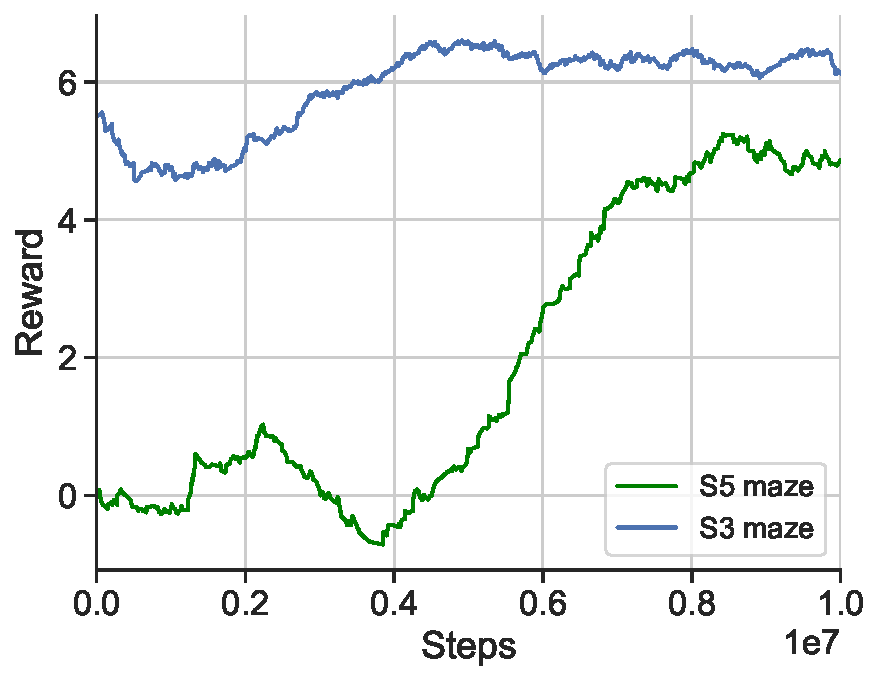
\includegraphics[width=0.8\linewidth]{figures/understanding_vsn/S3_S5_reward}
    \caption{\textbf{Learning curves for Maze-S3 and Maze-S5.} These curves show that the bigger the maze, the higher the complexity. On Maze-S3 the agent already starts at the saturation value around 6.5, but for Maze-S5 the agent needs more steps until it reaches its peak reward around a value of 5.}
    \label{fig:reward-maze-results}
\end{figure}

\begin{figure}
    \centering
    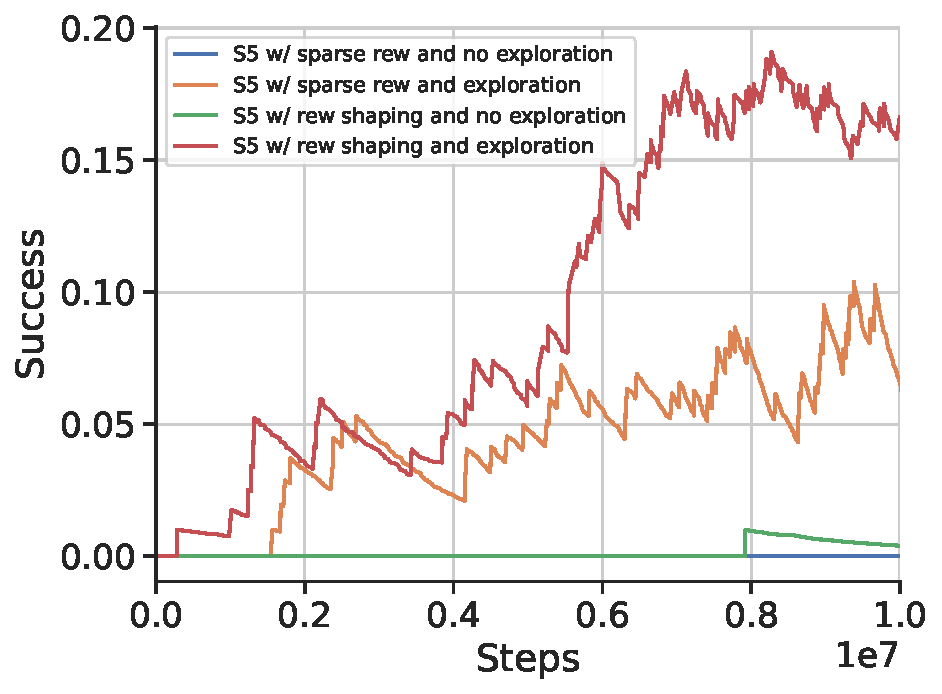
\includegraphics[width=0.8\linewidth]{figures/understanding_vsn/S5_ablation_success}
    \caption{\textbf{Ablation study on Maze-S5 during learning process.} Curves show that the best success rate is obtained using reward shaping and exploration techniques.}
    \label{fig:ablation-maze-success}
\end{figure}

\begin{table}
    \centering
    \scalebox{0.88}{\begin{tabular}{c c c c c c}
        \toprule
        Output type                                        & Maze         & Success                  & SPE               & Reward                   \\
        \midrule
        \multirow{2}{*}{Ours $+\; \epsilon\text{-}greedy$} & $S3$ & \textbf{0.75 $\pm$ 0.44} & \textbf{120.59 $\pm$ 111.85} & \textbf{6.80 $\pm$ 2.29} \\
        & $S5$ & \textbf{0.18 $\pm$ 0.38} & 534.40 $\pm$ 130.20          & \textbf{5.24 $\pm$ 5.73} \\

        \multirow{2}{*}{Ours $+\; stochastic$}             & $S3$ & 0.63 $\pm$ 0.49          & 127.42 $\pm$ 132.98          & 6.59 $\pm$ 2.41          \\
        & $S5$ & 0.17 $\pm$ 0.38          & \textbf{521.39 $\pm$ 182.66} & 5.14 $\pm$ 5.70          \\

        \multirow{2}{*}{$random$}                          & $S3$ & 0.18 $\pm$ 0.39          & 278.04 $\pm$ 51.55           & 0.37 $\pm$ 3.66          \\
        & $S5$ & 0.02 $\pm$ 0.14          & 596.07 $\pm$ 32.83           & -2.09 $\pm$ 4.06         \\
        \bottomrule
    \end{tabular}}
    \caption{\textbf{Evaluation performance for the best models on 100 test mazes.} We compare the evaluation between using $\epsilon\text{-}greedy$ with $\epsilon=0.2$ and using an \textit{stochastic} output, \ie, sampling actions from the last layer of the agent. In both mazes the best result is obtained with $\epsilon\text{-}greedy$.}
    \label{tab:results-maze}
\end{table}

\begin{table}
    \centering
    \scalebox{0.77}{\begin{tabular}{c c c c c c}
        \toprule
        Reward function            & Exploration strategy     & Success                  & SPE               & Reward                   \\
        \midrule
        \textit{distance reward}   & $\epsilon\text{-}greedy$ & \textbf{0.18 $\pm$ 0.38} & \textbf{534.40 $\pm$ 130.20} & \textbf{5.24 $\pm$ 5.73} \\
        \textit{navigation reward} & $\epsilon\text{-}greedy$ & 0.09 $\pm$ 0.29          & 575.86 $\pm$ 91.94           & 0.08 $\pm$ 0.26          \\
        \textit{distance reward}   & No                       & 0.02 $\pm$ 0.14          & 588.66 $\pm$ 79.78           & -1.24 $\pm$ 4.18         \\
        \textit{navigation reward} & No                       & 0.00 $\pm$ 0.00          & 600.00 $\pm$ 0.00            & 0.00 $\pm$ 0.00          \\
        \bottomrule
    \end{tabular}}
    \caption{\textbf{Ablation study for S5 mazes on 100 test mazes.} The results show that the best performance is obtained when \textit{distance reward} and $\epsilon\text{-}greedy$ techniques are used.}
    \label{tab:ablation-study}
\end{table}

\begin{figure}
    \centering
    \begin{subfigure}[b]{0.4\textwidth}
        \centering
        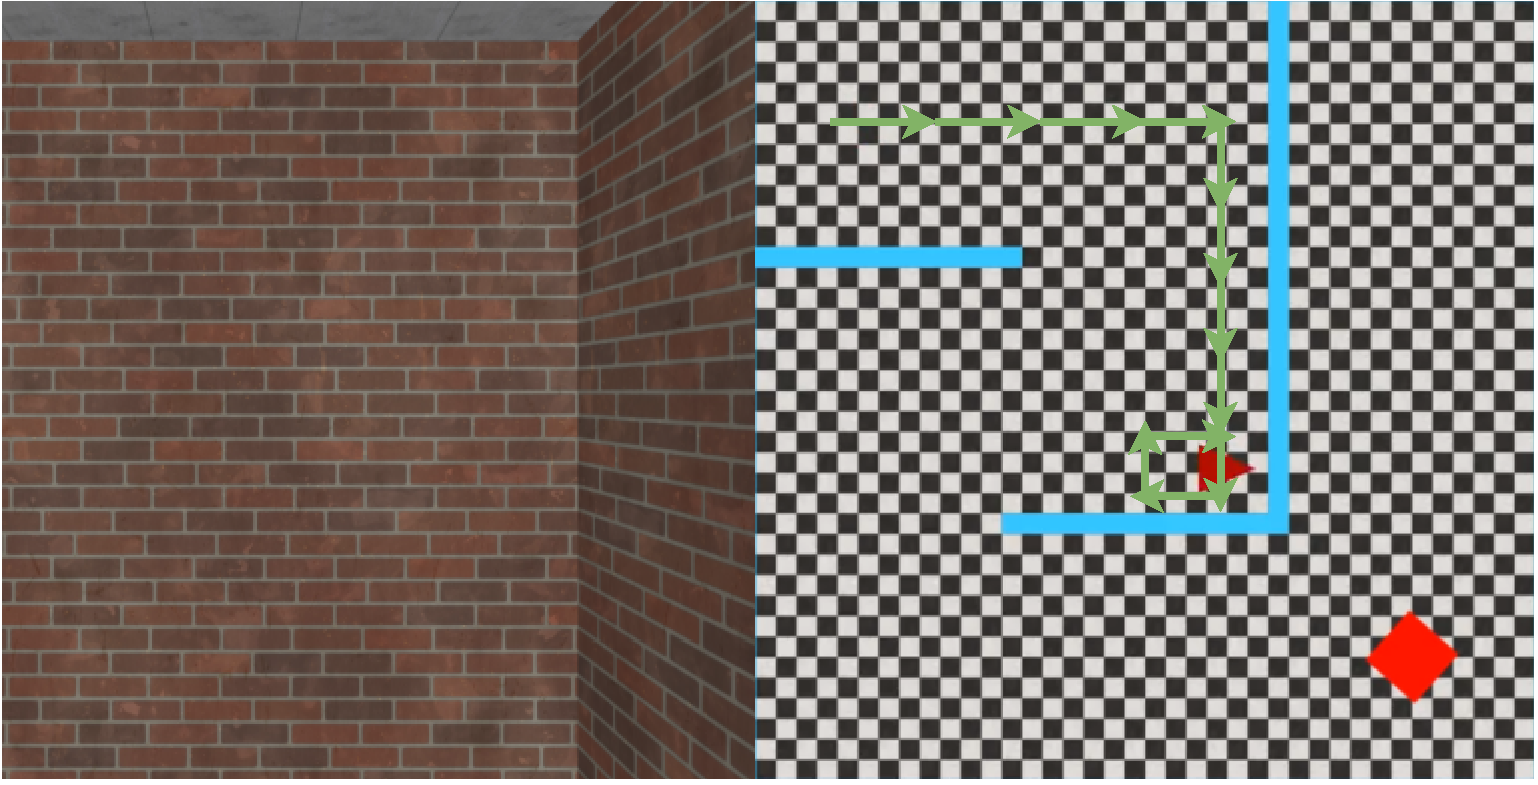
\includegraphics[width=0.8\textwidth]{figures/understanding_vsn/qualitative_results/fail}
        \caption{Failure case.}
        \label{fig:maze_qualitative_fail}
    \end{subfigure}
    \hfill
    \begin{subfigure}[b]{0.4\textwidth}
        \centering
        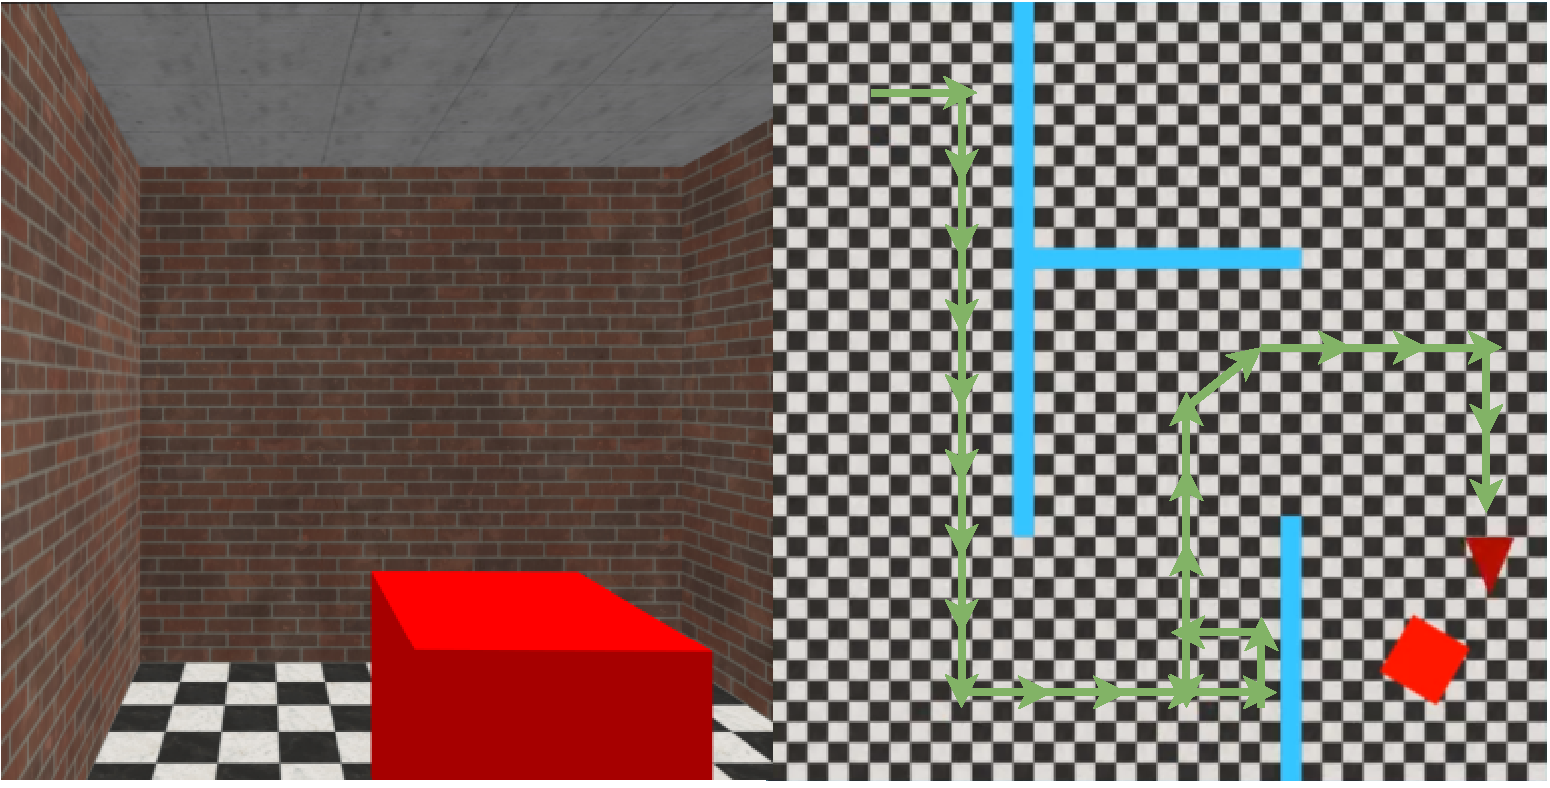
\includegraphics[width=0.8\textwidth]{figures/understanding_vsn/qualitative_results/success}
        \caption{Success case.}
        \label{fig:maze_qualitative_success}
    \end{subfigure}~\caption{\textbf{Qualitative results for Miniworld-Maze agent.} We show agent final state and trajectory for a fail case (\ref{fig:maze_qualitative_fail}) and a success case (\ref{fig:maze_qualitative_success}). In the success case, $\epsilon\text{-}greedy$ forces the agent to select a random action, thus exploring the environment, escaping the corner and finally reaching the target.}
    \label{fig:maze_qualitative}
\end{figure}

\subsection{Habitat results}\label{subsec:habitat-results}
Experiments in the Habitat benchmark enable us to assess how an agent would act in a more realistic scenario than the one presented by the mazes.
The agent has to navigate through the 3D scanned scene shown in figure~\ref{fig:dollhouse}.
The agent is initialized from random positions, and aims to locate one of the chairs present in the environment.

Figure~\ref{fig:reward-habitat-results} shows the reward obtained by the agent during the training process.
The first million steps correspond to an early stage of exploration.
Then, the reward quickly grows until the agent behavior becomes stable after 3 million steps.
%Compared with the learning curve for Maze-S5 in figure~\ref{fig:reward-maze-results}, both learning process are similar.

Table~\ref{tab:results-habitat} shows a comparison between our best agent under the same two different output options as in the previous experiment ( $\epsilon\text{-}greedy$ with $\epsilon=0.2$ and \textit{stochastic}), and a random agent as control case.
Results show how the $\epsilon\text{-greedy}$ approach reports a success rate of $96\%$, while the $\text{stochastic}$ output approach only reaches the target $73\%$ of the times.

Figure~\ref{fig:habitat_qualitative} provides qualitative results for our agent.
It shows the final state (left image) and the top view with the agent's trajectory in blue.
These figures clearly show how in both cases a different valid goal is reached (the agent reaches two different chairs) and how the $\epsilon\text{-greedy}$ strategy leads the agent to do coarser movements.

\begin{table}
    \scalebox{0.7}{\begin{tabular}{c c c c c c}
        \toprule
        Output type                       & Success                  & SPL              & DTG               & SPE               & Reward                   \\
        \midrule
        Ours $+\; \epsilon\text{-}greedy$ & \textbf{0.96 $\pm$ 0.19} & \textbf{$0.66 \pm 0.25$}  & \textbf{$0.25 \pm 0.85$}   & \textbf{189.99 $\pm$ 116.97} & \textbf{4.96 $\pm$ 1.99} \\
        Ours $+\; stochastic$             & $0.73 \pm 0.45$          & $0.58 \pm 0.36$  & $0.63 \pm 1.17$   & $231.23 \pm 188.13$          & $3.52 \pm 3.90$          \\
%        Ours $+\; deterministic$          & $0.13 \pm 0.33$         & $0.12 \pm 0.30$  $ $2.72 \pm 1.57$   & $432.57 \pm 161.40$          & $-2.03 \pm 3.84$         \\
        $random$                          & $0.05 \pm 0.22$          & $0.02 \pm 0.10$  &$4.49 \pm 1.72$    & $495.50 \pm 26.96$           & $-4.68 \pm 2.16$         \\
        \bottomrule
    \end{tabular}}
    \caption{\textbf{Best agent performance on 100 test episodes in Habitat.} The $\epsilon\text{-greedy}$ output mode reports the best results.}
    \label{tab:results-habitat}
\end{table}

\begin{figure}
    \centering
    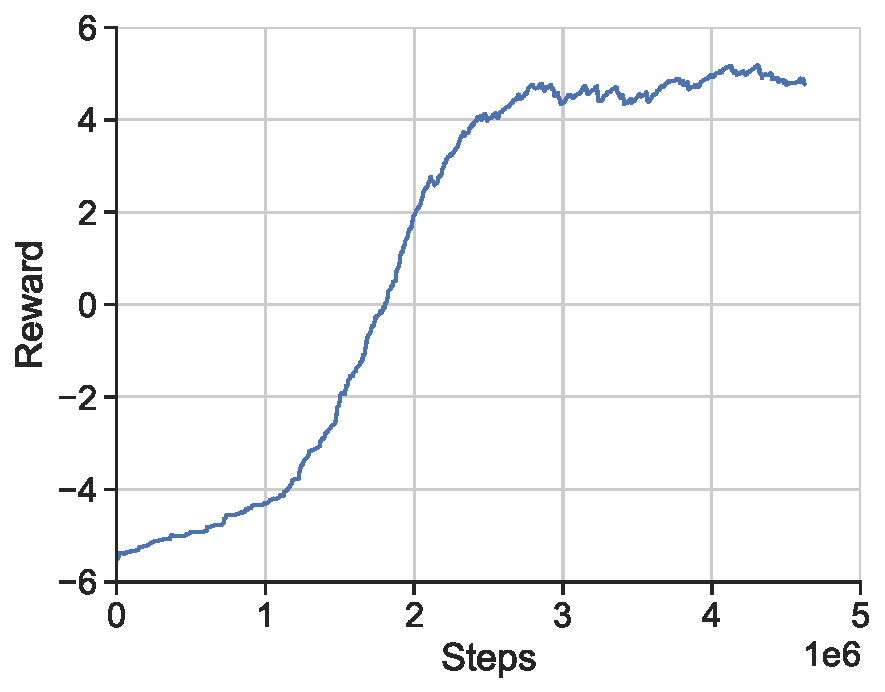
\includegraphics[width=0.7\linewidth]{figures/understanding_vsn/habitat_reward}
    \caption{\textbf{Learning curve of Habitat experiment.} This curve shows how the agent starts with a sub-optimal policy, receiving low rewards around $-5$. Then, the rewards increase until a value around 5, once the agent gets an optimal policy.}
    \label{fig:reward-habitat-results}
\end{figure}

\begin{figure}
    \centering
    \begin{subfigure}[b]{0.4\textwidth}
        \centering
        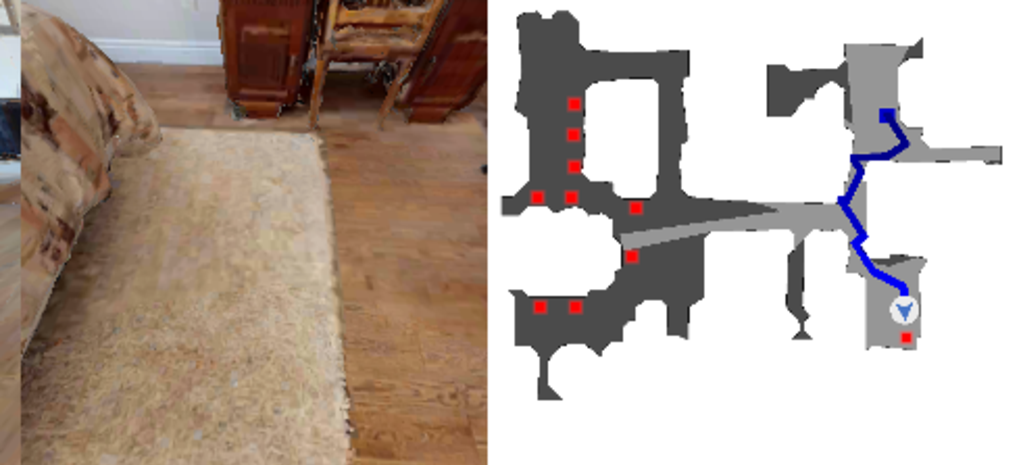
\includegraphics[width=\textwidth]{figures/understanding_vsn/qualitative_results/habitat_epsilon}
        \caption{$\epsilon\text{-greedy}$ output.}
        \label{fig:habitat_qualitative_epsilon}
    \end{subfigure}
    \hfill
    \begin{subfigure}[b]{0.4\textwidth}
        \centering
        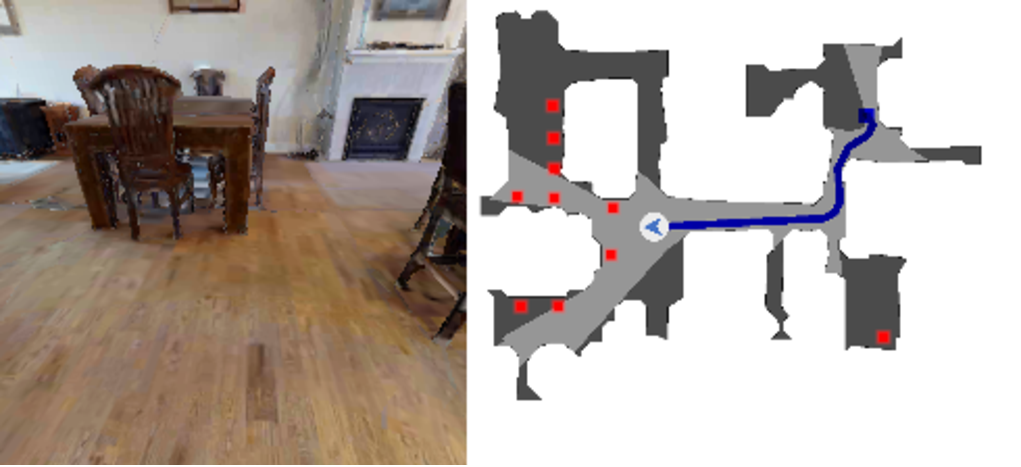
\includegraphics[width=\textwidth]{figures/understanding_vsn/qualitative_results/habitat_stochastic}
        \caption{$Stochastic$ output.}
        \label{fig:habitat_qualitative_stochastic}
    \end{subfigure}~\caption{\textbf{Qualitative results for Habitat agent.} Here we show the agent final state and trajectory on the scene using $\epsilon\text{-greedy}$ with $\epsilon = 0.2$ (\ref{fig:habitat_qualitative_epsilon}) and $stochastic$ output (\ref{fig:habitat_qualitative_stochastic}). Note that the $stochastic$ output produces a smother trajectory.}
    \label{fig:habitat_qualitative}
\end{figure}

\begin{figure}    
    \centering
    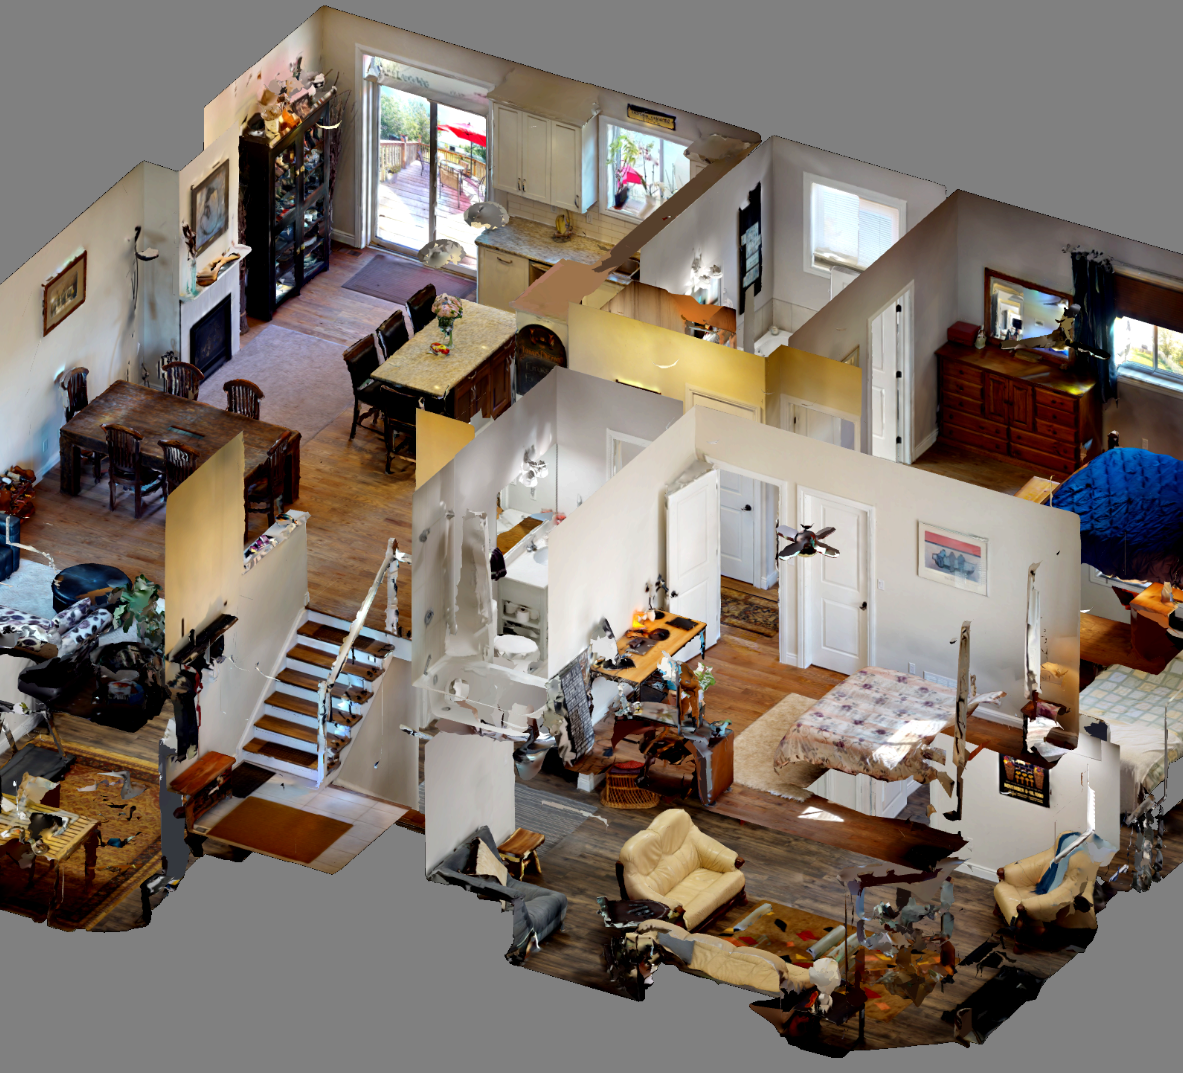
\includegraphics[width=0.6\linewidth]{figures/understanding_vsn/dollhouse}
    \caption{\textbf{Scene 00744-1S7LAXRdDqK from HM3D dataset.} Scene used for Habitat experiments.}
    \label{fig:dollhouse}
\end{figure}
